 \documentclass[CMPE]{KGCOEReport}

\usepackage{float}
\usepackage{graphicx}
\usepackage{amsmath}
\usepackage{kmap}
\newcommand{\classCode}{CMPE 160}  
\newcommand{\name}{Christopher Larson}
\newcommand{\LabSectionNum}{L3}
\newcommand{\LabInstructor}{Mr.\ Dominguez}	
\newcommand{\TAs}{Andrew Ramsey \\ Matthew Millar \\ Madeline Mooney}
\newcommand{\LectureSectionNum}{01}
\newcommand{\LectureInstructor}{Professor Beato}
\newcommand{\exerciseNumber}{05}
\newcommand{\exerciseDescription}{Combinational Logic Circuit Design Using Boolean Algebra Simplification }
\newcommand{\dateDone}{7 February 2018}
\newcommand{\dateSubmitted}{14 February 2018}

\begin{document}
\maketitle

\section*{Abstract}
The objective of the exercise was to apply combinational logic design to the implementation of two different equations. The two equations used in the exercise were found using Karnaugh Maps to simplify a Boolean expression into the POS and SOP form. The POS and SOP forms were then used as a guideline to build a circuit, the waveforms of this circuit was compared to the waveforms of a given testbench. The use of a testbench was important to validating the correct of the circuit, the circuit was found to be correctly built as the waveforms of the testbench and the circuit were identical.

\section*{Design Methodology}
The Boolean expression used to create the sum of products and product of sums expressions was $F = \Sigma_{ABCD} (0,2,3,4,6,7,13,14,15)$. The Karnaugh map representations of the expressions are shown in Figure 1 for the $F_{SOP}$ and Figure 2 for the $F_{POS}$. For the SOP expression the "1"s in the K-map are circled and for the POS expression the "0"s are circled.


\begin{figure}[H]
	\centering
	\begin{Karnaugh}[A][B][C][D]
		\contingut{1,0,1,1,1,0,1,1,0,0,0,0,0,1,1,1}
		\implicant[2pt]{7}{14}{blue}
		\implicantLateral[2pt]{0}{6}{red}
		\implicant[2pt]{3}{6}{green}
		\implicant[2pt]{13}{15}{black}
		\end{Karnaugh}
		\caption{K-map of $F_{SOP}$}
		\label{fig:Figure 1}
\end{figure}

The equation given from the K-map in Figure 1 is shown in Equation 1. This is the sum of products equation with the minimal amount of terms.

\begin{equation} F_{SOP} = \overline{A}C + BC + \overline{A}\,\overline{D} + ABD \end{equation}
\begin{figure}[H]
	\centering
	\begin{Karnaugh}[A][B][C][D]
		\contingut{1,0,1,1,1,0,1,1,0,0,0,0,0,1,1,1}
		\implicant[2pt]{1}{5}{blue}
		\implicant[2pt]{8}{10}{red}
		\implicant[2pt]{12}{8}{green}
		\end{Karnaugh}
		\caption{K-map of $F_{POS}$}
		\label{fig:Figure 2}
\end{figure}

The equation given from the K-Map in Figure 2 is shown in Equation 2. This is the product of sums equation with the minimal amount of terms.

\begin{equation} F_{POS} = (A + C + \overline{D})(\overline{A} + B)(\overline{A} + C + D) \end{equation}\\

Using Equations 1 and 2, a circuit diagram was drawn to represent both equations of expression F. This circuit diagram is shown in Figure 3, both expressions use the same inputs but go to different outputs represented as $F_{SOP}$ and $F_{POS}$.

\begin{figure}[H]
	\centering
	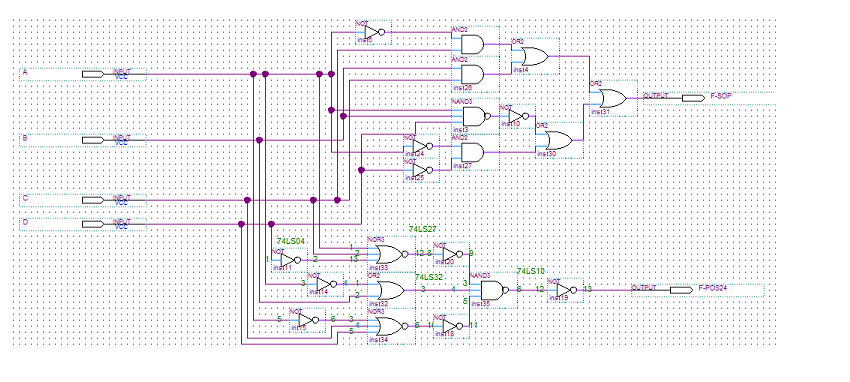
\includegraphics[width=1.00\textwidth]{QuartusL5}
	\caption{The circuit diagram for the SOP and POS forms of the function F}
	\label{fig:Figure 3}
\end{figure}

The circuit diagram in Figure 3 was used to model the waveform of the equation with the least amount of chips and the least amount of EGC, or equivalent gate count. The equation with the least was the POS equation, with a total of 9 EGC and the use of 4 chips.

\section*{Results and Analysis} 

The waveform in Figure 4 matched the waveform in the test bench exactly and shows the circuit design was correct. Since the POS and SOP equations were derived from the same expression and are equal to each other, the waveforms of the two are identical. The waveform also confirms that the equations were derived correctly, and that the circuit diagram was constructed correctly.

\begin{figure}[H]
	\centering 
	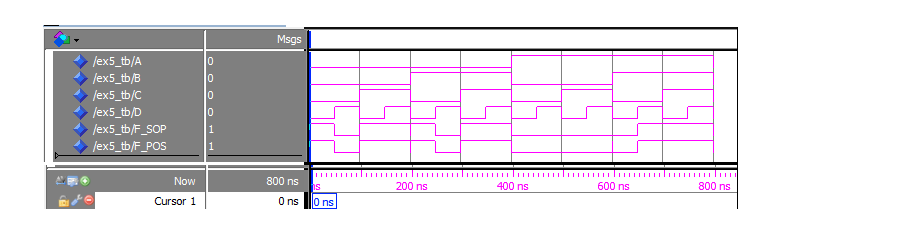
\includegraphics[width=1.20\textwidth]{ModelsimL5}
	\caption{The ModelSim representation of function F}
	\label{fig:Figure 4}
\end{figure}
 
\section*{Conclusion}

The use of K-maps to simplify an expression into the minimal POS and SOP equation is helpful when trying to create a circuit that uses the least amount of chips and the lowest equivalent gate count. It is important to simulate the simplified equations to ensure that the outputs are equivalent to the original Boolean expression and to each other. The exercise proved successful as the testbench, POS and SOP waveforms were all identical.

\section*{Questions}
1.
\begin{figure}[H]
	\centering
	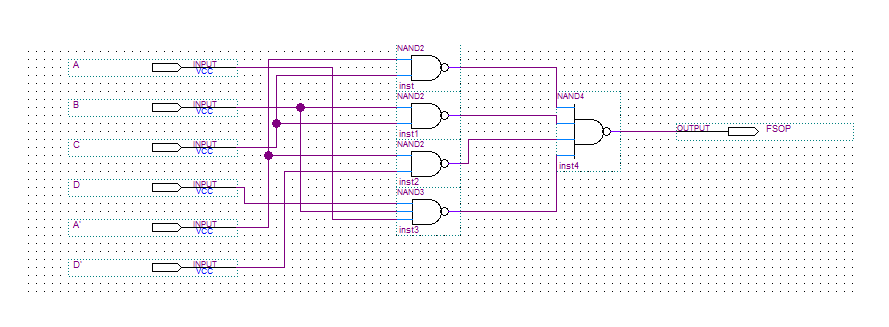
\includegraphics[width=1.00\textwidth]{QuartusL5Q1}
	\caption{Question 1: 2-level NAND-NAND implementation}
	\label{fig:Figure 5}
\end{figure}

2.
\begin{figure}[H]
	\centering
	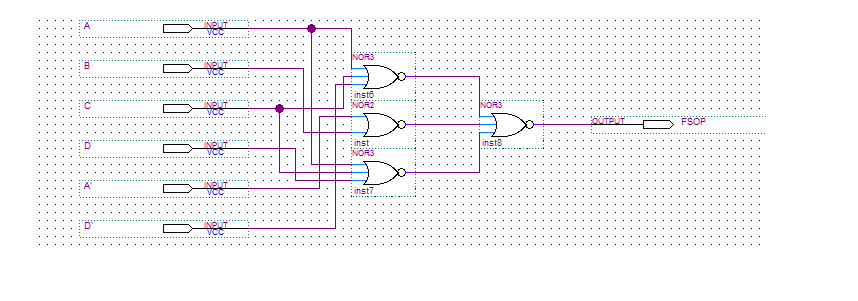
\includegraphics[width=1.10\textwidth]{QuartusL5Q2}
	\caption{Question 2: 2-level NOR-NOR implementation}
	\label{fig:Figure 6}
\end{figure}


\end{document}